\section{Characterizing OLED Power Draw on Modern Phones}
\label{sec:measurement}

% Nexus 6, Pixel 2, and Moto Z3 from three recent generations
An accurate OLED power model for modern smartphones must
capture any unique OLED power draw behavior on such
devices. Therefore, we start with a measurement study to characterize
the OLED power draw behavior on three modern smartphones.

%  We used NEXUS 6, Moto Z3 and Pixel 2 with our low overhead Android
%  app.  It generates the average current consumed when an image is
%  displayed on the OLED screen.  We captured the current consumed by a
% monochromatic image i.e. all pixels having the same RGB values.
%
\paragraph{Methodology.}
We conduct our study on three smartphones from three recent
generations, Pixel 2, Moto Z3, and Pixel 4,
released in 2017, 2018, and 2019, respectively, as listed in
Table~\ref{tab:phones}.

\begin{table}[tp]
\centering
\caption{{OLED displays in the 3 phones used in our study.}}
\label{tab:phones}
\vspace{-0.1in}
{\scriptsize
          \begin{tabular}{|c|c|c|c|c|c|}
          \hline
          Phone   & OLED display & Resolution  & \makecell{Base\\power} & \makecell{Dark Screen\\power} & \makecell{Android\\ Version} \\
          \hline
          Pixel 2 & AMOLED       & 1080 x 1920 & 22.9 mA  & 43.2 mA  & R (11) \\ 
          Moto Z3 & Super AMOLED & 1080 x 2160 & 21.4 mA  & 57.6 mA  & Pie (9) \\ 
          Pixel 4 & AMOLED       & 1080 x 2280 & 23.6 mA  & 78.8 mA  & R (11) \\
          \hline
          \end{tabular}
}
\vspace{-0.2in}
\end{table}

\forjnl{
  \begin{figure}[tp]
	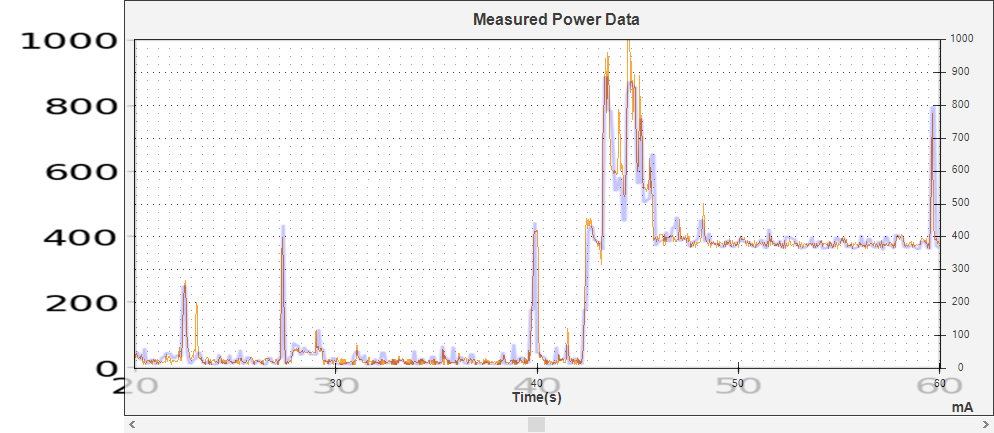
\includegraphics[width=0.45\textwidth]{./figure/1400_base_cpu_idle.png}
	\caption{Stable phone power draw on Nexus 6 during screen-off
          with CPU idle (left half) and 
          during displaying a static image (right half);
         (2) Instantaneous power sensor reading (blue)
         matches with power meter readings (yellow).
        }
	\label{fig:base_current}
        \vspace{-0.2in}
\end{figure}
}

\begin{figure*}[tp]
	\begin{subfigure}[]{0.31\textwidth}
		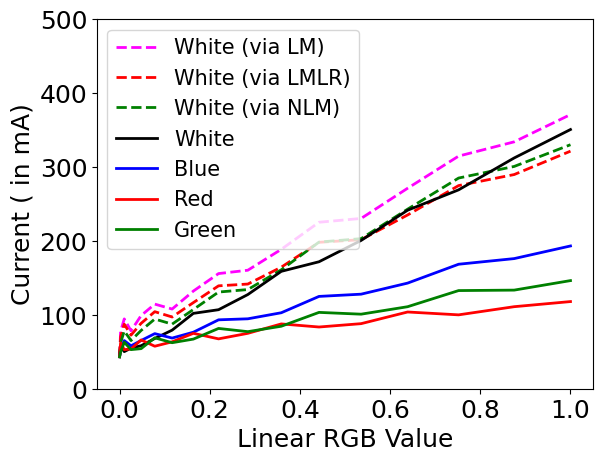
\includegraphics[width=\textwidth]{figure/002_Pixel2_linear_model.png}
		\caption{Pixel 2}
		\label{fig:initial_evaluation_2_n6_w}
	\end{subfigure}
	\hfill
	\begin{subfigure}[]{0.31\textwidth}
		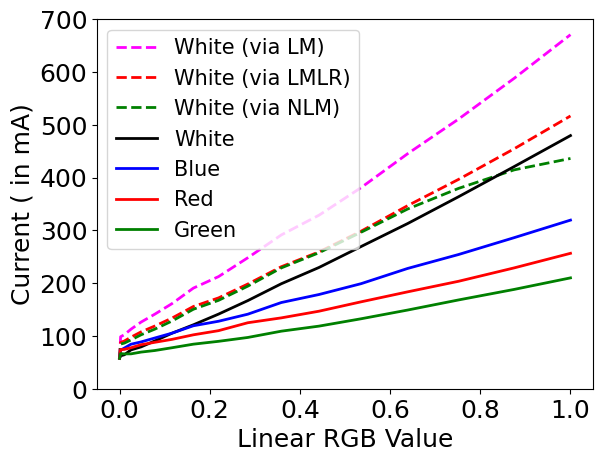
\includegraphics[width=\textwidth]{figure/003_MotoZ3_linear_model.png}
		\caption{Moto Z3}
		\label{fig:initial_evaluation_2_p2_w}
	\end{subfigure}
	\hfill
	\begin{subfigure}[]{0.31\textwidth}
		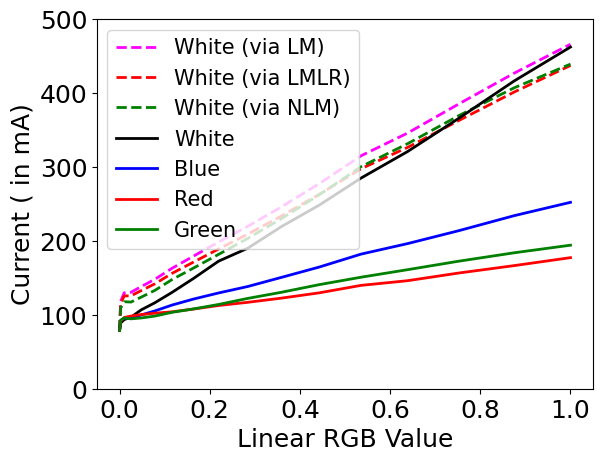
\includegraphics[width=\textwidth]{figure/004_Pixel4_linear_model.png}
		\caption{Pixel 4}
		\label{fig:initial_evaluation_2_z3_w}
	\end{subfigure}
\vspace{-0.1in}
	\caption{OLED display power in displaying one-color images on three phones (with default color mode).
		(LM: linear model as in Eqn.~\ref{eq:linear_equation},
subt		 LMLR: linear model with linear regression, NLM: Non-Linear Model).
}
        \vspace{-0.1in}
        \label{fig:initial_evaluation_2}
\end{figure*}

To accurately measure the phone power draw in our experiments, 
% \eg in displaying a static image, 
we directly connect each of the three
phones to a Monsoon power monitor~\cite{powermonitor}
which has a current sampling rate of 5 KHz.

To facilitate measurements of OLED display power for different colored
pixels, we created a simple Android app that displays a static image
at a time on the screen, while the phone power draw is being measured.
The images used will have the same dimension as the screen, \eg
1920x1080 pixels on Pixel 2.
%    \dtext{Periodically we displayed a black screen where all the pixel
%      values were set to zero and recorded black screen power draw. To get
%      the power draw by colored pixels we subtracted this black screen
%      power from the color static image power draw .}
% To isolate the OLED display power,
%    To isolate the dark screen power, we measure the phone power while
%    the static image is displayed and when the screen is off but CPU is
%    idle (using a wakelock).
First, we measure the CPU idle power 
as the power power draw when the screen is off and the CPU is idle using a wakelock.
Second, we measure the OLED dark screen power 
by displaying a dark screen with all the pixel values set to zero
(during which time the CPU is 99\% idle)
and then subtract the CPU idle power (from Step 1) from the measured phone power.
Finally, to measure the power draw by all the colored pixels,
\ie {$\sum_{i=0}^{n}{P_i}$} in Eqn.~1,
in displaying a staic image (during which time the CPU is also 99\% idle),
 we subtract both the dark
screen power and the CPU idle power
from the phone power measured in displaying the color static image.
%   \forjnl{Figure~\ref{fig:base_current} shows example power meter readings
%   of the two power values.}
\if 0
Since in displaying a static image, the CPU
is 99\% idle and no other phone component is used, the difference
between the two measurements can be attributed to the OLED display power.
\fi

% For easy-of-use,
% our methodology uses built-in power sensor for the actual power measurement.  Since
% the power sensors have relatively coarse resolution, 170ms, 1.4s, and 1.4s, for
% the three phones respectively, we make the app display each image for
% 5 to 10 seconds to gather multiple power sensor readings and use the average as
% the ground truth.


\if 0
Nexus 6, we directly connected the phone to a Monsoon current
Monitor (FTA33D)~\cite{monsoon} to measure the power draw.  For Pixel
2 and Moto Z3 Plus, we used the in-built current sensor to measure the
phone current draw.  To avoid the noise from transient power
fluctuation in displaying a new image, the app displays each image for
5 seconds, during which period the CPU and GPU utilization stays less
than 2\%, and hence the
total power draw consumed by the phone can be attributed to the OLED
display.
\fi

% Since the current sensor reading resolution
% on the two phones are coarse (1.5 seconds), we extend the duration of displaying
% each image to 40 seconds to allow more current
% sensor readings and hence high fidelity in the measured current.

\if 0
\subsection{Pixel Independence}
\label{subsec:basic}

We first validate the two basic assumptions behind
Eqn.~\ref{eq:linear_equation0}.  We make the app display three sequences of
images, each with an increasing percentage of red, green, or blue colored
pixels (with RGB value 255)
respectively, between 0\% and 100\%.  Figure~\ref{fig:basic} shows that (1)
the OLED display draws a non-zero power for dark screen -- this is the
base power $C$, which differ slightly across the 3 phones (Table~\ref{tab:phones}).
\footnote{A major contributor to the base OLED power comes
comes from the touchscreen sensor embedded in the
display~\cite{touchscreenpower}.}
\footnote{In this paper, for power
  measurement we directly report the power using the current drawn, in
  milli-Amperes (mA).  The actual power consumed would be the current
  drawn multiplied by 3.7V, the voltage supply of the battery.}
%
(2) the OLED power draw grows linearly with the percentage
of non-dark pixels of each color -- the
linear curves intersect at RGB value 0.
These results confirm the two
basic assumptions in Eqn.~\ref{eq:linear_equation0}.

%  The same assumptions are made in all previous studies of OLED
%   (\eg~\cite{dong2009current,kim2013runtime}).

\begin{figure}[tp]
        \vspace{-0.1in}
        % \includegraphics[width=0.45\textwidth]{./figure/1500_Horizontal.pdf}
        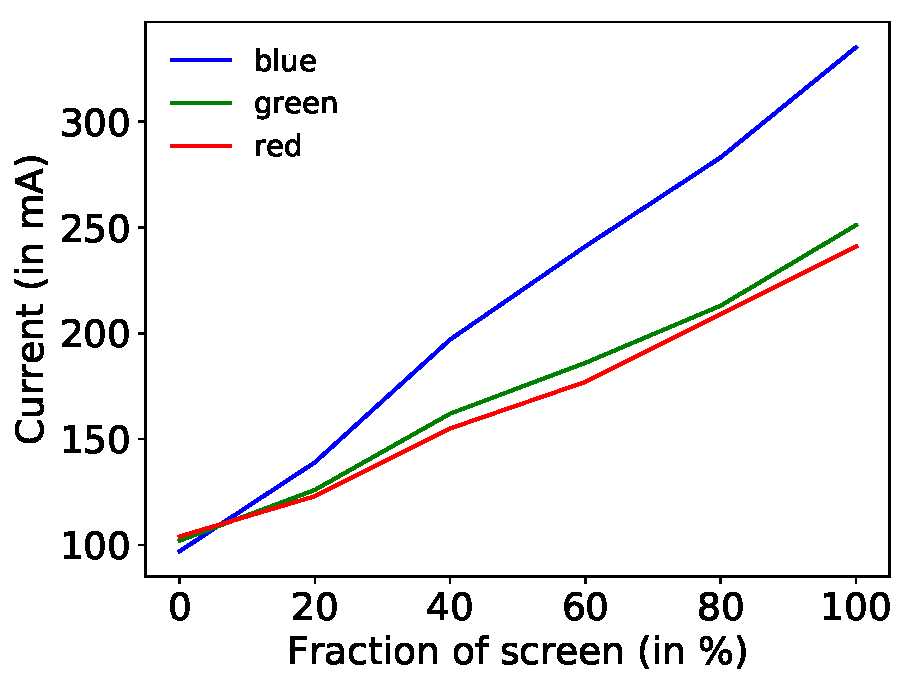
\includegraphics[width=0.30\textwidth]{./figure/1501_Vertical.pdf}
        \vspace{-0.1in}
	\caption{OLED display power under varying percentage of non-dark pixels on Nexus 6.}
        \vspace{-0.1in}
        \label{fig:basic}
\end{figure}

Given that the above two assumptions hold, the remaining challenge
in OLED power modeling
is how to capture the power draw by each pixel $P_i$ as a function of the RGB
values of that pixel ($R_i, G_i,B_i$).

The simplest approach is to measure and tabulate
the power draw of all possible RGB values. This is infeasible
due to the large number of color combinations ($256^3$=16M on modern phone OLED displays).

Since each pixel of OLED display consists of 3 subpixels corresponding
to the three base colors, the most natural approach is to measure the
power draw of each subpixel $f(R_{i})$, $g(G_{i}$, and $h(B_{i})$ as a
function of the color intensity (256$\times$3 measurements), and derive the pixel power
draw for any RGB value as a function of the subpixel power functions:
\begin{equation}
	P_i(R_i, G_i,B_i) = M(f(R_{i}), g(G_{i}), h(B_{i}))
	\label{eq:linear_equation1}
\end{equation}
Subpixel models $f(R_{i})$, $g(G_{i})$ and $h(B_{i})$ can be
trained by displaying monochromatic images on the screen.  For
example, $f(R_{i})$ is obtained as the power in displaying all pixels
in the screen with color ($R_{i}$, 0, 0), minus base power $C$,
and normalized by the total number of pixels.

To gain insight on how to develop the model function $M$,
we next study a few basic properties of the OLED power behavior.

\fi

\subsection{Superposition Property}
\label{subsec:super}

The first question we ask is whether the power draw of the three
subpixels are independent, \ie whether they satisfy the {\em superposition
property} which states that the power consumed by three subpixels are
additive.

\paragraph{Methodology.}
To validate the superposition property, 
we measure the OLED power consumed by
7 monochromatic images containing 3 base colors (red, green, blue),
3 2-channel colors (yellow, magenta and cyan)
and the 3-channel color white, with varying intensities (sRGB values from 0 to 255).

\if 0
\dcomment {
Figures~\ref{fig:initial_evaluation_2}(a)--\ref{fig:initial_evaluation_2}(c)
show the measured OLED display power.
%   for the three base colors and white, and the
%   sum of the power for the three base colors label ``White (via LM)'',
%   on the three phones.
Due to the gamma-correction in sRGB standard,
the subpixel power draw is known to be nonlinear in the sRGB values.
Thus in this paper, we transform the sRGB format into the linear format, known as Linear RGB~\cite{gammaCorrection1} ({$Linear RGB = (sRGB/256)^{2.2}$}),
%  Thus in this paper, we transform the sRGB format into the linear format, known as Linear RGB~\cite{gammaCorrection1},\footnote{$Linear RGB = (sRGB/256)^{2.2}$.}
and plot all OLED power functions w.r.t. Linear RGB values.
Figures~\ref{fig:initial_evaluation_2}(a)--\ref{fig:initial_evaluation_2}(c) show that
(1) the subpixel power draw for the 3 base colors are linear in the Linear RGB values;
(2) the subpixel power draw are not additive -- 
the gap between their sum (without duplicating base power)
and the measured power draw for white
widens with the color intensity,
reaching 2\%, 45\%, and 0.5\% at linear RGB value 1.0 (sRGB value of 255)
for the three phones, respectively.

\forjnl{Figures~\ref{fig:initial_evaluation_2}(d)-\ref{fig:initial_evaluation_2}(f)
  show}

We performed the same analysis for the 2-channel color magenta
(figures not shown due to page limit). Again, we
observe a large deviation between the sum of the power for blue and
red and the actual measurement; the gap widens with the color
intensity, reaching 7\%, 25\%, and 6\% at linear RGB value 1.0 for
the three phones, respectively.  The corresponding gaps are 7\%, 15\%, and 0.8\% for
yellow and 3\%, 17\%, and 2\% for cyan for the three phones.
These results show that
%
{\em subpixel powers are not additive.} The likely reason is that the
  subpixels utilize common driving circuits within the display
  hardware module.
  
CHANGED THIS BECAUSE THE MAXIMUM ERROR IS NOT AT Linear RGB 1.0}
\fi

\paragraph{Findings.}
{
Figures~\ref{fig:initial_evaluation_2}(a)--\ref{fig:initial_evaluation_2}(c)
show the measured OLED display power. Due to the gamma-correction in sRGB standard,
the subpixel power draw is known to be nonlinear in the sRGB values.
Thus in this paper, we transform the sRGB format into the linear format, known as Linear RGB~\cite{gammaCorrection1} ({$Linear RGB = (sRGB/256)^{2.2}$}),
and plot all OLED power functions w.r.t. Linear RGB values.
Figures~\ref{fig:initial_evaluation_2}(a)--\ref{fig:initial_evaluation_2}(c) show that
(1) the subpixel power draw for the 3 base colors are linear in the Linear RGB values;
(2) the subpixel power draw are not additive -- 
the difference between their sum (without duplicating base power)
and the measured power draw for white
varies across the color intensity, reaching
a maximum of 92\%, 66\% and 43\% at
0 (14), 0.04 (59) and 0.01 (25) linear RGB values (sRGB values) for the 3 phones, respectively.
% widens for Moto Z3 with color intensity but decreases for Pixel 2 and Pixel 4.
% widens with the color intensity,
% 1.0 (sRGB value of 255)
% reaching 2\%, 45\%, and 0.5\% at linear RGB value 1.0 (sRGB value of 255)
% for the three phones, respectively.
% \comment{THE GAP IS TOO SMALL FOR P2 and P4. DOES THIS NEEDS TO CHANGE?}

\forjnl{Figures~\ref{fig:initial_evaluation_2}(d)-\ref{fig:initial_evaluation_2}(f)
  show}

We performed the same analysis for the 2-channel color magenta
(figures not shown due to page limit). Again, we
observed a large deviation between the sum of the power individually observed for blue and
red compared to the actual measurement; the gap
% widens with
varies across the color intensity, reaching
55\%, 45\% and 26\% at 0.05 (64), 0.05 (67) and 0.01 (27) linear RGB values (sRGB values)
% at linear RGB value 1.0
for the three phones, respectively.
Simillar gaps are also observed for yellow, \eg of
60\%, 16\% and 18\% at 0.05 (68), 0.10 (91) and 0.02 (43) linear RGB values (sRGB value),
and for cyan, of
44\%, 17\% and 21\% at 0.0 (19), 0.23 (130) and 0.01 (34) linear RGB values (sRGB values),
for the three phones, respectively.
These results show that
%
{\em subpixel powers are not additive.} The likely reason is that the
  subpixels utilize common driving circuits within the display
  hardware module.
}
  
\subsection{Monotonicity Property}
\label{subsec:monoproperty}

We next study whether a more basic property holds in the OLED power
behavior on modern phones.  The {\em monotonicity property} is stated
as follows:

\noindent
{\bf Monotonicity property:}
The OLED pixel power draw for RGB value ($x_1, y_1, z_1$)
is less than that for ($x_2, y_2, z_2$) iff
vector ($x_1, y_1, z_1$) is canonically less than ($x_2, y_2, z_2$),
\ie $x_1 \leq x_2$, $y_1 \leq y_2$, and $z_1 \leq z_2$.

\paragraph{Methodology.}
To validate the monotonicity property, we measure the OLED power draw
in displaying monochromatic images generated by sweeping the 3-D RGB
color space, with each base color intensity varied from 0 to 255 (in
the sRGB space) in steps of 16 (and including value 255) for a total
of 17$^3$ images. We then compare the display power
draw for each pair of adjacent RGB values in the
17$\times$17$\times$17 grid of discretized 3-D color space.



% \begin{figure*}[tp]
% 	\begin{subfigure}[]{0.31\textwidth}
% 		\includegraphics[width=\textwidth]{./figure/275_N6_monotonicity_cube.pdf}
% 		\caption{Nexus 6}
% 		\label{fig:initial_monotonicity_n6_w}
% 	\end{subfigure}
% 	\hfill
% 	\begin{subfigure}[]{0.31\textwidth}
% 		\includegraphics[width=\textwidth]{./figure/277_P2_monotonicity_cube.pdf}
% 		\caption{Pixel 2}
% 		\label{fig:initial_monotonicity_p2_w}
% 	\end{subfigure}
% 	\hfill
% 	\begin{subfigure}[]{0.31\textwidth}
% 		\includegraphics[width=\textwidth]{./figure/276_Z3_monotonicity_cube.pdf}
% 		\caption{Moto Z3}
% 		\label{fig:initial_monotonicity_z3_w}
% 	\end{subfigure}
% 	\caption{The OLED display current showing monotonicity not being
% 		followed on three phones. (Best see in Color)}
% \label{fig:initial_monotonicity}
% \end{figure*}


\paragraph{Findings.}
Interestingly, on all three phones, we found many instances of power
measurements that violate the monotonicity property.  Table~\ref{tab:initial_evaluation_3} lists a few samples for each of the 3
phones, where each row lists the power draw for two color vectors, the
second being canonically larger yet drawing less power than the first.
For example, on Pixel 4, the OLED power draw for RGB value (32, 16, 16) should
be higher than that for (32, 0, 16). Instead,
our measured value for the former, 89mA, 
is 1.09X
lower than that for the later, 97mA.
Since this pattern happens on all three phones,
it is unlikely due to manufacturing defect.
We conjecture\footnote{We could not find any white papers from the OLED vendors
  or the driver source code which are all proprietary.}
that the reasons for the above non-monotonicity behavior
{are two-fold:
(1) there may be OEM-specific color transformation performed
in the hardware composer (Figure~\ref{fig:arch}) that alters the canonical
order of sRGB values;
and
(2) the subpixels utilize
common driving circuits within the display hardware module
differently at different color intensities.
}


\begin{table}[tbp]
	\centering
	\caption{Sample RGB value pairs for which the OLED display
          power violates the monotonicity property.}
        \vspace{-0.1in}
          {\small
          \begin{tabular}{ | l||l|r||l|r| }
		\hline
		Type & Color 1 & Current & Color 2 &  Current \\
                & & (mA) & & (mA) \\
		\hline
                \multicolumn{5}{c }{Pixel 2} \\
		\hline
		1 chl to & ( 176, 0, 0) & 91 & ( 176, 0, 64) & 83 \\
		 2 chl & ( 0, 96, 0) & 79 & ( 0, 96, 16) & 70 \\
		 & ( 0, 0, 16) & 56 & ( 0, 16, 16) & 48 \\
		\hline
		2 chl to & ( 112, 192, 0) & 146 & ( 112, 192, 32) & 131 \\
		 3 chl & ( 112, 0, 80) & 82 & ( 112, 16, 80) & 68 \\
		 & ( 0, 48, 48) & 71 & ( 48, 48, 48) & 53 \\
		\hline
		\multicolumn{5}{c }{Moto Z3} \\
		\hline
		1 chl to & ( 240, 0, 0) & 230 & ( 240, 0, 64) & 225 \\
		 2 chl & ( 0, 224, 0) & 254 & ( 0, 224, 32) & 247 \\
		 & ( 0, 0, 192) & 135 & ( 16, 0, 192) & 133 \\
		\hline
		2 chl to  & ( 240, 240, 0) & 378 & ( 240, 240, 80) & 357 \\
		3 chl & ( 192, 0, 224) & 246 & ( 192, 48, 224) & 220 \\
		 & ( 0, 160, 224) & 242 & ( 64, 160, 224) & 215 \\
		\hline
		\multicolumn{5}{c }{Pixel 4} \\
		\hline
		1 chl to  & ( 80, 0, 0) & 105 & ( 80, 0, 32) & 100 \\
		2 chl & ( 0, 240, 0) & 233 & ( 32, 240, 0) & 230 \\
		 & ( 0, 0, 224) & 173 & ( 16, 0, 224) & 172 \\
		\hline
		2 chl to & ( 128, 16, 0) & 113 & ( 128, 16, 16) & 109 \\
		3 chl  & ( 32, 0, 16) & 97 & ( 32, 16, 16) & 89 \\
		 & ( 0, 176, 192) & 234 & ( 16, 176, 192) & 229 \\
		\hline
	\end{tabular}
         }
	 \label{tab:initial_evaluation_3}
\end{table}

% \begin{figure*}[tp]
% 	\begin{subfigure}[]{0.27\textwidth}
% 		\includegraphics[width=\textwidth]{./figure/401_n6_err.png}
% 		\caption{Nexus 6}
% 	\end{subfigure}
% 	\begin{subfigure}[]{0.27\textwidth}
% 		\includegraphics[width=\textwidth]{./figure/403_p2_err.png}
% 		\caption{Pixel 2 Saturated Color Mode}
% 	\end{subfigure}
% 	\begin{subfigure}[]{0.27\textwidth}
% 		\includegraphics[width=\textwidth]{./figure/402_z3_err.png}
% 		\caption{Moto Z3}
% 	\end{subfigure}
% 	\begin{subfigure}[]{0.10\textwidth}
% 		\includegraphics[width=\textwidth]{./figure/404_err_bar.png}
% 		\caption{Error Bar}
% 	\end{subfigure}
% 
% 	\caption{Prediction error of the linear modeling for the 3-D RGB color space, for all RGB values $(r, g, b)$ where $r, g, b$ are multiples of 16.}
% 	\label{fig:error_wrt_linear}
% \end{figure*}


% We found out how the error varies with respect to the linear model (i.e.
% Equation\ref{eq:linear_equation}) in the color space. The main observation
% is that as we go father away from the (0,0,0) the error increases. In Nexus 6
% we observed that the highest error is observe in the center of the color space.
% This reinforced our conviction that we require a more robust model to cater
% to the OLED display current estimation in mobile phones.

% We start by validating the previous liner OLED current model
% (Eqn~\ref{eq:linear_equation}) via measurements on three phones, Nexus
% 6 (Android Nougat 7.1.1), Pixel 2 (Android 9.0), and Moto Z3 (Anroid
% 9.0), which all have OLED display.
% 
% For Nexus 6, we directly connected the phone to a Monsoon current
% Monitor (FTA33D)~\cite{monsoon}. We created a simple Android app that
% displays one static image at a time on the screen. The images were
% created to have the same dimension as the screen (\eg 2560x1440 pixels
% on Nexus 6). Four series of mono-colored images were displayed,
% corresponding to red, green, blue and white, respectively.
% In each series, consecutive images differ from each other by 10 units of RGB
% value. To avoid the noise from transient current fluctuation in
% displaying a new image, the app displays each image for 5 seconds,
% during which period the CPU and GPU utilization stays less than 1\%
% and the total current consumed by the phone is attributed to the OLED
% display.
% 
% Figure~\ref{fig:initial_evaluation}(a) shows the measured OLED diplay
% current with varying intensities for the 4 mono colors on Nexus 6.
% We make the following observations.
% (1) The blue color  draw far more current than red/green, by 24\% at RGB value of 256;
% (2) The white color only draw marginally more current than blue, by 24\% at RGB value of 256;
% (3) The white color draws far less current than the summation of
% those by red, green and, blue, separately, by 52\% at RGB value of 256, which
% would be the error for the simple linear model.
% 
% We repeated the experiment using Pixel 2 and Moto Z3 Plus using the in-built
% current sensor to measure the phone current draw. Since the current sensor reading resolution
% on the two phones are coarse (1.5 seconds), we extend the duration of displaying
% each image to 40 seconds to allow more current
% sensor readings and hence high fidelity in the measured current.
% 

\subsection{Impact of Brightness Level}
\label{subsec:brightness}

Modern smartphones come with a hardware button or software brightness
slider that allows users to directly adjust the display brightness
level, \eg between 0\% -- 100\%.  We found that {\em brightness level
  adjustment by either scheme does not change frame pixel values
  recorded in the frame buffer}, 
suggesting that some color transformation
caused by the slider brightness level happens after the frame
buffer, \ie in the hardware composer (Figure~\ref{fig:arch}). 
Hence an OLED power model based on the frame pixel values needs to be
adjusted for the display brightness level.
However, our measurements also showed that 
the OLED display power draw does not scale linearly in displaying a same image
with the slider brightness level.

% From reading AOSP source code~\cite{sourcecode:brightness1,sourcecode:brightness2},
We searched the kernel exported hardware info \comment{is this accuract to say?}
and  found that for Android Pie and later vesions, % (\eg Pixel 2 and Moto Z3),
the brightness slider value (0\% to 100\%) is 
%   not linearly correlated with 
transformed to the system screen brightness value (0 to 255),
which can be read from system variable {\small \tt
  /sys/class/leds/lcd-backlight/brightness} on Pixel 2 and Moto Z3
and {{\small \tt /sys/class/backlight
    /panel0-backlight/brightness} on Pixel 4}.  
Second, we experimentally 
% correlated the two brightness levels and 
found that the slider brightness level is mapped 
to the system brightness level via a logarithmic function.
%   Moto Z3 and Pixel 4 by plotting the brightness slider value and 
%   system variable that would lead to the same OLED power draw.
as shown in Figure~\ref{fig:brightnessslider_brightnesslevel}.
Finally, we experimentally confirmed that the OLED display current
scales linearly with the system brightness value in displaying the 7
monochromatic colored images (3 base colors, 3 2-channel colors and
white).

\forjnl{as shown in Figure~\ref{fig:brightnessslider_brightnesslevel}.
}

Our above findings have two implications.
First, when recording a frame as an input to the OLED power model,
we also need to record the system brightness level so that
the output of the pixel value-based power prediction
can be scaled linearly to the system brightness level.
Second, OLED display power at a reduced slider brightness level (\eg 30\%)
actually drains much less power (\eg 9/255 = 3.5\% for Pixel 4 as shown in Figure~\ref{fig:brightnessslider_brightnesslevel}), due to the logarithmic relationship
between the two (slider and system) brightness levels.


\if 0
Modern smartphones come with a hardware button or software brightness
slider that allows users to directly adjust the display brightness
level, \eg between 0\% -- 100\%.  We find that {\em brightness level
  adjustment via either scheme does not change frame pixel values
  recorded in the frame buffer}, suggesting some color transformation
caused by slider brightness level change happens after the frame
buffer, \ie in the hardware composer (Figure~\ref{fig:arch}). 
%  Thus any OLED power model based on the frame pixel values has to
%  explicitly take into account the actual display brightness level.
Furthermore, our measurements show that 
the OLED display power draw in displaying a same image
does not scale linearly with th slider brightness level.

From reading AOSP source code~\cite{sourcecode:brightness1,sourcecode:brightness2},
we found that for Android Pie and later vesions % (\eg Pixel 2 and Moto Z3),
the brightness slider value (between 0\% and 100\%) is 
%   not linearly correlated with 
converted to the system screen brightness value (between 0 and 255)
which can be read from system variable {\small \tt
  /sys/class/leds/lcd-backlight/brightness} on Pixel 2 and Moto Z3
and {{\small \tt /sys/class/backlight
    /panel0-backlight/brightness} on Pixel 4}.  Instead, the mapping
in a logarithmic scale.  The logarithmic scaling follows the XDA
Analysis~\cite{brightness2019} which explains that human eyes observe
noticeable intensity changes in a logarithmic manner.
% the change in the brightness slider (from linear to logarithmic ) is due to the Weber's Law (i.e. the noticeable change.)
%
% This follows the Weber law~\cite{weber} logarithmic property.
%  Earlier with linear scale, it was observed that about 90\% of the brightness was controlled
%  by only left 20\% of the slider~\cite{brightness2019}.
%  Now with the add logarithmic support
%  changes in screen brightness are much more noticeable to human eye
%  when the screen is dark versus when the screen is bright.
We experimentally confirmed this logarithmic brightness level mapping on Pixel 2,
Moto Z3 and Pixel 4 by plotting the brightness slider value and 
system variable that would lead to the same OLED power draw.
\comment{why do we need to do this? cannot we verify by 
reading the two values directly?}
Figure~\ref{fig:brightnessslider_brightnesslevel} shows that
the system brightness value is logarithmically related
with the brightness slider value.
%    To derive the empirical correlation
%    between the brightness slider value and the system variable, we set the variable
%    from 0 to 255 and observed the brightness slider.
%    and the system variable as shown in
%
% for Nexus 6, the two are linearly related whereas
% for Pixel 2 and Moto Z3,
%   The system variables values are 89, 9 \& 11 for 30\% brightness
%   and 136, 22 \& 24 for 50\% brightness
%   for the Nexus 6, Pixel 2 \& Moto Z3 receptivity.
Uncovering this correlation for a given device allows us to calculate
the OLED display power for any brightness slider value.

Finally, we confirmed that
the OLED display current scales linearly with
the system brightness value
% variable {\small \tt /sys/class/leds/lcd-backlight/brightness}
in displaying
%  varied this value in steps of 10 and noted the current drawn separately on
the 7 monochromatic colored images (3 base colors, 3 2-channel colors and white).
The results are omitted due to page limit.
\fi
% We observed that the display current changes linearly,
\forjnl{as shown in Figure~\ref{fig:brightnesss_phones}.
  }

%% To derive the empirical correlation
%% between the brightness slider value and the actual brightness level
%% after color transformation (sent to hardware display), we manually
%% set the system variable /sys/class/leds/lcd-backlight/brightness 0
%% to 255 in increments of 10 and record the display power draw.
%% Similarly, we manually
%% adjust the brightness slider from 0\% to 100\% with increments of 10\%
%% and record the display power draw,
%% in displaying each of the 7 
%% % (3 base colors, 3 2-channel colors and white)
%% monochromatic colored images.
%% We then plot the corresponding values between the slider
%% and the actual brightness level which results in the same display power draw in
%% Figure~\ref{fig:brightnessslider_brightnesslevel}.  We observe
%% indeed that on Nexus 6, the two metrics are lineared related,
%% but on Pixel 2 and Moto Z3, the actual brightness level scales
%% with the logrithmic of the slide values.
%   that at different brightness level is mapped to brightness slider for
%   the phones.  (The orange line is for 30\% and purple like is for 50\%
%   brightness slider levels.)  We also observe that this relationship is
%   not affected by change in the color modes.


\begin{figure}[tb]
	\centering
	\begin{subfigure}[]{0.31\textwidth}
		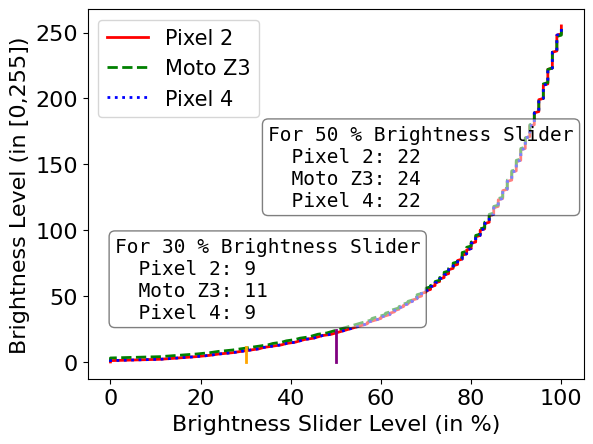
\includegraphics[width=\textwidth]{figure/brightness_curve.png}
	\end{subfigure}
        \vspace{-0.1in}
	\caption{Relationship between the slider brightness level and the system brightness
		value.}
	\label{fig:brightnessslider_brightnesslevel}
\end{figure}

%% With the above unstanding of theslider value, 
%% in Figure~\ref{fig:brightnesss_phones}, we show how the OLED current varies with the
%% actual brightness level.
%% We observe that it follows a linear relationship on all three phones.
%% For Pixel 2 and Moto Z3, we observe that OLED power consumption decreases comparatively
%% more than Nexus 6.
%% In Nexus 6 the brightness slider starts with brightness level 17. This the reason
%% for the sharp drop in the brightness level in Figure~\ref{fig:brightnessslider_brightnesslevel}.
%% Similarly as there the current remain constant for lower value of brightness level
%% in Figure~\ref{fig:brightnesss_phones_n6}.
%% We so conclude that the display power is linearly
%% proportional to the actual brightness level.
%% We use a lookup from brightness slider to the actual brightness level
%% to model their correlation for each phone.

\if 0
\begin{figure*}[tp]
	\begin{subfigure}[]{0.31\textwidth}
		\includegraphics[width=\textwidth]{./figure/a1111_N6_brightness_corrected.pdf}
		\caption{Nexus 6}
		\label{fig:brightnesss_phones_n6}
	\end{subfigure}
	\hfill
	\begin{subfigure}[]{0.31\textwidth}
		\includegraphics[width=\textwidth]{./figure/a1112_P2_brightness_corrected.pdf}
		\caption{Pixel 2}
	\end{subfigure}
	\hfill
	\begin{subfigure}[]{0.31\textwidth}
		\includegraphics[width=\textwidth]{./figure/a1111_Z3_brightness_corrected.pdf}
		\caption{Moto Z3}
	\end{subfigure}
        \vspace{-0.1in}
	\caption{OLED current with varying brightness level for the three phones.
		(The black screen base current is removed.)}
	\label{fig:brightnesss_phones}
\end{figure*}
\fi

\if 0
the OLED power draw are linear in terms of RGB values gamma-corrected
with the brightness level,
as shown in Figures~\ref{fig:brightnesslevel}(c) for Pixel 2,
and captured in Eqn.~(\ref{eq:brigthness_equation_2}:
\begin{equation}
  P_i(R_i, G_i, B_i, Br) = P_i( Br^{2.2}\cdot R_i, Br^{2.2}\cdot G_i, Br^{2.2}\cdot B_i, 1.0)
  \label{eq:brigthness_equation_2}
\end{equation}
where
%$Br$ is the brightness level between 0 to 1 and
$P_i(R_i, G_i, B_i, Br)$ is the pixel power
for RGB value $(R_i, G_i,B_i)$ at brightness level $Br$.
For example, if we
display a white screen with RGB value of (255,255,255) with 80\%
brightness, the display power will be equivalent to having the RGB
value gamma-corrected with the brightness level, \ie (156,156,156)
since $0.8^{2.2}*255=156$. We believe this new
  interpretation of brightness level is a policy change 
that happened starting from {Android O}.
  \fi

  
% \begin{figure}[tp]
% %  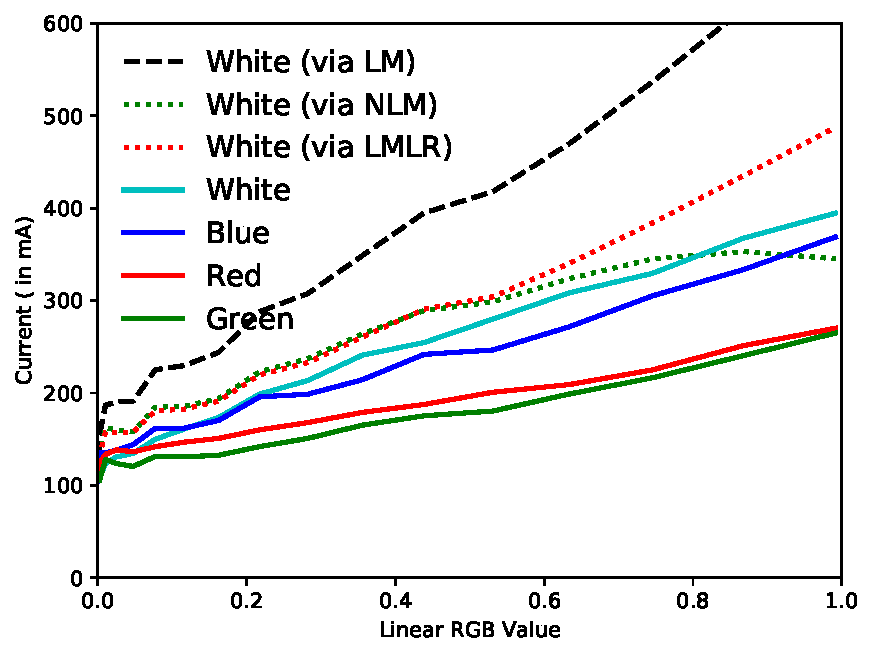
\includegraphics[width=\textwidth]{./figure/240a_n6_standard.pdf}
%         \vspace{-0.1in}
% 	\caption{OLED display power under varying the brightness level.}
%         \vspace{-0.1in}
%         \label{fig:brightnesslevel}
% \end{figure}

% \begin{figure*}[tp]
% 	\begin{subfigure}[]{0.31\textwidth}
% 		\includegraphics[width=\textwidth]{./figure/1100_N6_brightness.pdf}
% 		\caption{Nexus 6}
% 	\end{subfigure}
% 	\begin{subfigure}[]{0.31\textwidth}
% 		\includegraphics[width=\textwidth]{./figure/1122_P2_brightness_with_correction.pdf}
% 		\caption{Pixel 2}
% 	\end{subfigure}
% 	\begin{subfigure}[]{0.31\textwidth}
% 		\includegraphics[width=\textwidth]{./figure/1102_P2_brightness.pdf}
% 		\caption{Pixel 2: with gamma correction}
% 	\end{subfigure}
%         \vspace{-0.1in}
% 	\caption{OLED power draw is linear in the brightness level on Nexus 6 but
%           linear in the brightness-gamma-corrected RGB colors on Pixel 2 and Moto Z3 (not shown).}
% 	\label{fig:brightnesslevel}
% \end{figure*}

% \begin{figure*}[tp]
% 	\begin{subfigure}[]{0.31\textwidth}
% 		\includegraphics[width=\textwidth]{./figure/1100_N6_brightness.pdf}
% 		\caption{Nexus 6}
% 	\end{subfigure}
% 	\begin{subfigure}[]{0.31\textwidth}
% 		\includegraphics[width=\textwidth]{./figure/1102_P2_brightness.pdf}
% 		\caption{Pixel 2}
% 	\end{subfigure}
% 	\begin{subfigure}[]{0.31\textwidth}
% 		\includegraphics[width=\textwidth]{./figure/1101_Z3_brightness.pdf}
% 		\caption{Moto Z3}
% 	\end{subfigure}
%         \vspace{-0.1in}
% 	\caption{OLED power draw is linear in the brightness level on Nexus 6 but
%           nonlinear on Pixel 2 and Moto Z3.}
% 	\label{fig:brightnesslevel}
% \end{figure*}

% To understand the impact of the brightness level on the OLED power
% draw, we measure the OLED power draw by displaying monochromatic
% images of 7 colors: 3 base colors, 3 2-channel colors and white, as
% the display brightness level is adjusted in steps of 20\% using the brightness slider.
% Figures~\ref{fig:brightnessslider_brightnesslevel}(a)-(c) show that
% {\em
% for Nexus 6, the OLED power scales linearly with the brightness level,
% but for Pixel 2  and Moto Z3, the OLED power draw scales linearly
% at low brightness levels but turns exponentially
% at high brightness levels. ??is thisstill true???
% }

%   \comment{
% curve fitting and
%   we found that since Android O, Android interprets 
%   screen brightness level as some intricate color transformation
%   that is not easily described in a simple function.
%   }
%

\subsection{Impact of Color Mode and Color Correction}
\label{subsec:colortransform}

In addition to the brightness level, we found two other forms of color transformation
can happen in recent versions of Android.
First, Android Lollipop introduced 
{\em color correction} for visually impaired users~\cite{colorcorrection}.
% , which also uses HardwareComposer to change the color actually displayed.
%  Color correction comes with 3 modes: Deuteranomaly (red-green),
Second, Android 8.1 Oreo added templates for adding new {\em color modes}.
%with the help of HardwareComposer2~\cite{colormode}
%  which uses HardwareComposer2~\cite{colormode} to perform color
%  transformation to change the color displayed.
% It requires factory calibration data, stored in the device, to adjust variation in manufacturing.
OEMs can use this template mechanism to display vibrant colors by utilizing
the wide color gamut.
\forjnl{For example, Pixel 2 phones provide 3 color modes:
Natural, Boosted (default) and Saturated,
and Moto Z3 phones come with 2 color modes, Standard and Vibrant (Default), and
Vibrant has 3
variations, namely, Warm, Neutral (Default) and Cool.
Figure~\ref{fig:initial_evaluation_color_mode} in Appendix A2
shows that the OLED power draw in displaying the same monochromatic images 
for non-default color modes on Pixel 2 and Moto Z3 differ from
those in Figure~\ref{fig:initial_evaluation_2}.
}
%  Protanomaly (red-green), and Tritanomaly (blue-yellow).

Both color change features are implemented by passing a color
matrix~\cite{colormatrix} to the hardware composer, which performs the
color transformation on the frame pixels before sending them to the
display. In doing so,
they alter the OLED power draw without changing
the frame buffer recorded, similarly as with brightness level adjustment.
{For example, our measurments have shown (results omitted due to page limit)
  that on Pixel 2, displaying the same
  white-color image under Natural and Saturated Color Modes
draws 2.6\% and 4.9\% more power than the default color mode.
}
% cannot catch such color-transformed pixels sent to the display, and hence
Hence, {\em OLED power models using frame buffer as input need to be derived
for each color mode or correction.}


